\documentclass[11pt,a4paper]{article}
\usepackage[T1]{fontenc}
\usepackage[utf8]{inputenc}
\usepackage{lmodern,microtype}
\usepackage[margin=.85in]{geometry}
\usepackage{amsmath,amssymb,mathtools}
\usepackage{booktabs,tabularx,array,enumitem,needspace,float}
\usepackage{xcolor,tikz}
\usetikzlibrary{arrows.meta,positioning,fit,calc}
\usepackage[hidelinks]{hyperref}
\usepackage[nameinlink,noabbrev]{cleveref}
\usepackage{fancyhdr}
\hypersetup{pdftitle={Sequencer Rotation: Architecture and Module Contracts},
pdfsubject={Architecture index compatible with Sync HotStuff RR v4.4}}
\pagestyle{fancy}\fancyhf{}
\lhead{\small Sequencer rotation architecture}\rhead{\small v4.4 baseline}
\cfoot{\thepage}\setlength{\headheight}{14pt}
\setlength{\parindent}{0pt}\setlength{\parskip}{4pt}
\setlength{\emergencystretch}{2em}
\setlist{nosep,leftmargin=*}
\newcolumntype{Y}{>{\raggedright\arraybackslash}X}
\newcommand{\api}[1]{\ensuremath{\mathsf{#1}}}
\newcommand{\Hash}{\mathsf H}
\newcommand{\GF}{\mathsf{GF}}
\newcommand{\RF}{\mathsf{RF}}
\newcommand{\FC}{\mathcal F}
\newcommand{\TB}{\mathit{TB}}
\newcommand{\role}{\textbf{Role and contract.}\ }
\newcommand{\iface}{\textbf{Minimal interface.}\ }
\newcommand{\depends}{\textbf{Dependencies and boundary.}\ }
% Source links are relative to the exported PDF in output/pdf/.
\newcommand{\src}[2]{\href{../../formalization_v2/#1}{\texttt{\detokenize{#2}}}}
\definecolor{ink}{HTML}{17324D}
\definecolor{blue}{HTML}{EAF1FA}
\definecolor{green}{HTML}{E8F3EE}
\definecolor{sand}{HTML}{FBF1DC}
\title{Sequencer Rotation\\[3pt]\large Architecture and Module Contracts}
\author{}\date{12 October 2026}

\begin{document}
\begin{center}
{\LARGE Sequencer Rotation\par}\vspace{5pt}
{\large Architecture and Module Contracts\par}\vspace{8pt}
12 October 2026
\end{center}
\begin{abstract}
The system provides an authorized stream of mini-block batches and binds
rollup publication to that stream. L1 manages participation and authority;
regional consensus orders batches and rotates leaders; cross-region
rotation and an honest monitoring service recover from regional failure.
Proposer $P$ publishes a contiguous globally final prefix, with the same
ordered input used for data availability and execution. This document is
the index and contract layer for those modules. Sync HotStuff RR v4.4 is
the consensus and Force baseline. New integration contracts are identified
explicitly; they are not claims that the complete system is already proved
or implemented.
\end{abstract}

\section{Service goals and module map}\label{sec:map}
The architecture has two end-to-end goals.
\begin{enumerate}
\item \textbf{Reliable sequencing.} Supply authentic, ordered batches with
an append-only globally final prefix. Under the stated progress conditions,
the prefix grows and its data reach live consumers. Regional output may be
consumed earlier, with the possibility of a Force replacing that suffix.
\item \textbf{Faithful publication.} Every accepted publication by $P$
extends the previously accepted prefix with exactly the next sequenced
input: no skipped batch, inserted transaction, changed order, or replayed
position. The DA data and execution claim refer to that same input.
\end{enumerate}
The second goal is an acceptance rule even when $P$ is Byzantine. Eventual
publication additionally needs an available proposer or a replacement
mechanism; a verifier cannot force an absent proposer to send data.

\begin{figure}[H]\centering
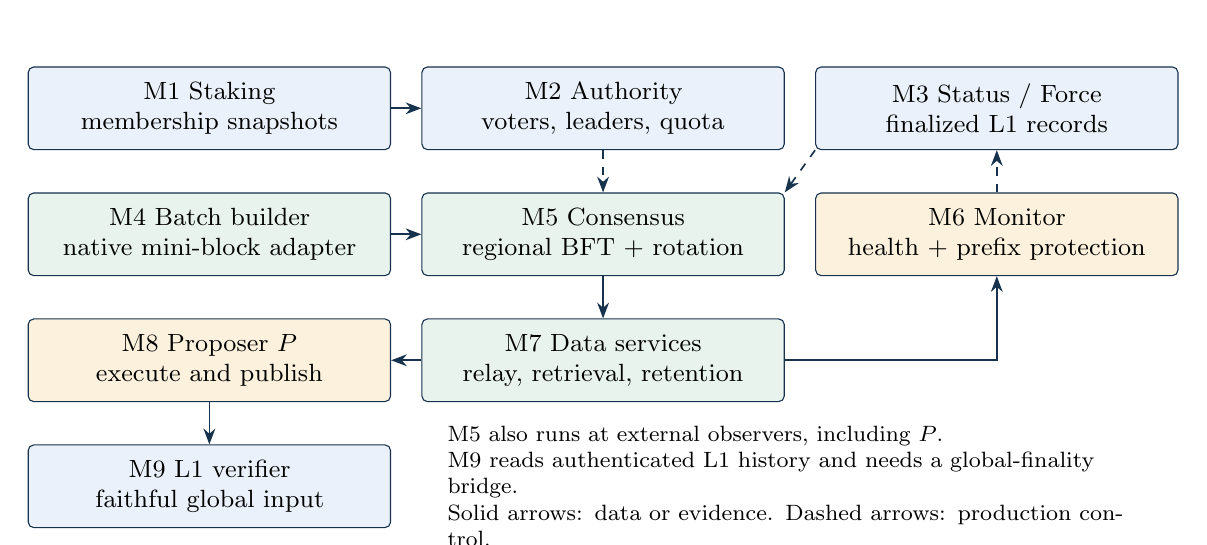
\begin{tikzpicture}[font=\small,
 box/.style={draw=ink,rounded corners=2pt,align=center,inner sep=5pt,
 text width=4.25cm,minimum height=1.05cm},
 arr/.style={-{Stealth[length=2mm]},semithick,draw=ink},
 ctl/.style={arr,dashed}]
\node[box,fill=blue] (stake) at (0,0) {M1 Staking\\membership snapshots};
\node[box,fill=blue] (auth) at (5.0,0) {M2 Authority\\voters, leaders, quota};
\node[box,fill=blue] (ctrl) at (10.0,0) {M3 Status / Force\\finalized L1 records};
\node[box,fill=green] (build) at (0,-1.6) {M4 Batch builder\\native mini-block adapter};
\node[box,fill=green] (cons) at (5.0,-1.6) {M5 Consensus\\regional BFT + rotation};
\node[box,fill=sand] (mon) at (10.0,-1.6) {M6 Monitor\\health + prefix protection};
\node[box,fill=green] (net) at (5.0,-3.2) {M7 Data services\\relay, retrieval, retention};
\node[box,fill=sand] (prop) at (0,-3.2) {M8 Proposer $P$\\execute and publish};
\node[box,fill=blue] (verify) at (0,-4.8) {M9 L1 verifier\\faithful global input};
\draw[arr] (stake)--(auth);
\draw[ctl] (auth)--(cons);
\draw[ctl] (ctrl.south west)--(cons.north east);
\draw[ctl] (mon)--(ctrl);
\draw[arr] (build)--(cons);
\draw[arr] (cons)--(net);
\draw[arr] (net)--(prop);
\draw[arr] (net.east)-|(mon.south);
\draw[arr] (prop)--(verify);
\node[align=left,text width=8.8cm,font=\footnotesize,anchor=west]
 at (2.9,-4.8) {M5 also runs at external observers, including $P$.\\
 M9 reads authenticated L1 history and needs a global-finality bridge.\\
 Solid arrows: data or evidence. Dashed arrows: production control.};
\end{tikzpicture}
\caption{Logical responsibilities. Modules may share a process or contract;
the separation identifies who establishes each property.}
\label{fig:architecture}
\end{figure}

M1--M3 and M9 are L1 services or services anchored in L1. M4--M5 run
at sequencers; M5's observer logic also runs at consumers. M6 is initially
one honest, coordinated multisignature service. M7 supplies communication
and data recovery. DA and execution verification are external rollup
services consumed by M8--M9, with explicit contracts below.

\section{Shared objects and the MegaETH boundary}\label{sec:objects}
\subsection{The few objects that cross modules}
One v4.4 \emph{DATA block} orders one batch of mini-blocks. Its DATA
height $h$ counts batches, not individual mini-blocks or EVM blocks.
One \emph{session} is one region's production turn; its views are
$(r,g,t)$, for session, recovery generation, and leader term.
The session opening identifies the branch as well as the numeric index
$r$. This matters because a Force may reuse $r$ on a different branch.

\begin{table}[H]\centering\small
\begin{tabularx}{\linewidth}{@{}p{.23\linewidth}Y@{}}
\toprule Object & Meaning at module boundaries\\\midrule
Voting snapshot $\mathit{cfg}$ & Region members, public keys and fixed
voting weights, with historical verification data.\\
Authority $\api{AUTH}_{r,g}$ & The snapshot, leader schedule and parameters
used by v4.4, including term cap $K$ and session quota $\TB_r$.\\
DATA block $B_h$ & A batch payload $x_h$, parent link, session context,
DATA/physical positions and finalized L1 reference $\rho$, as in v4.4.\\
Regional evidence $\pi_R(B)$ & A direct FINAL receipt $\FC_r(B)$, or a
covering same-session receipt and verified ancestry. A proposal QC is
insufficient.\\
Boundary witness $\mathcal W$ & REGULAR or FORCE opening, retained anchor
and its evidence, successor selection and finalized L1 proofs.\\
Checkpoint $C$ & A DATA prefix commitment and its height, opening
provenance, historical authority and processed L1 context.\\
Publication claim $y$ & Previous checkpoint, next input interval,
input/DA commitments and execution-state transition.\\\bottomrule
\end{tabularx}
\caption{Shared semantic objects; this is not a new wire format for v4.4.}
\label{tab:objects}
\end{table}

\subsection{Native mini-blocks and the ordering envelope}\label{sec:native}
The compatibility baseline is the local MegaETH specification at commit
\href{https://github.com/megaeth-labs/specification/tree/59797b45b1f59b7c2c147e6f99be39399a1f2b44}{\texttt{59797b45}}, especially
\src{../megaeth_specs/specs/protocol/blocks.md}{blocks.md} and
\src{../megaeth_specs/specs/protocol/state-sync.md}{state-sync.md}.
Its native mini-block header has eight fields, including transaction and
receipt roots, native positions and timestamps. It has no predecessor
hash or v4.4 L1 reference. A native mini-block belongs to exactly one
EVM block; the EVM transaction list concatenates its mini-block lists.
The public \href{https://docs.megaeth.com/mini-block}{Mini-Blocks guide},
checked on 12 October 2026, confirms the eight-field signing format and
EVM-boundary key changes.

The architecture preserves that native encoding. An \emph{ordering
envelope} is the v4.4 DATA block around an ordered payload
\[
 x_h=(M_{a_h},\ldots,M_{b_h}),\qquad
 \api{Input}(x_h)=\mathcal X_{a_h}\Vert\cdots\Vert\mathcal X_{b_h}.
\]
For empty DATA, both lists are empty.
The payload commitment binds each native header, exact transaction bytes,
mini-block boundary and position; native bodies additionally carry their
receipts. Here $\api{Input}(x_h)$ is the transaction projection;
the input commitment used for publication binds the full structured
payload, not only that projection. Batch ranges continue without gaps on
a branch. Parent links,
L1 control references and BFT authorization belong to the envelope.
No native timestamp is reinterpreted as an L1 height or a global-finality
clock. DRAIN is an internal consensus object and contributes no
mini-block, transaction, or EVM block.

\textbf{Native execution and signing.} Producing a full native mini-block
requires execution-derived receipts and gas information. An order-only
payload can be a separate integration mode, but is not already a native
mini-block. Regional consensus certifies the chosen ordered payload;
execution correctness needs the rollup execution check. BFT FINAL
signatures are also distinct from native header signatures and
transaction receipts.

The native signer is selected by \texttt{sequencerAt(EVM block number)}.
Thus changing a BFT leader is not automatically permission to change
the native signer midway through an EVM block. The published
\href{https://docs.megaeth.com/spec/system-contracts/sequencer-registry}
{SequencerRegistry specification}, checked on 12 October 2026, specifies
pre-block activation; its Rex6 version also requires a new-key possession
proof and a minimum scheduling delay. This is a specification check, not
a deployment claim.

M4 owns the adapter between BFT production authority and this native
signing rule. A compatible implementation keeps one authorized native
key per EVM block and supplies a valid execution continuation at handoff.
Decoupling that key from the current BFT leader is possible as an
architecture choice, but its availability must be provided. If the key
fails or a Force cuts within an EVM block, the adapter must specify how
the retained prefix can be continued and how the next key becomes
authorized. v4.4 does not supply that rule. An arbitrary mid-block key
replacement would require an explicit native-protocol change.

\section{L1 participation and control}\label{sec:l1}
\subsection{M1: Staking, membership and accountability}\label{sec:staking}
\role Admit stake-backed operators through public rules, queue joins and
exits, escrow slashable balances, and expose immutable voting snapshots.
Permissionless participation means eligibility is rule-based; it does not
mean a new deposit immediately changes an active BFT committee.

\iface
\[
 \api{Join}(\text{key},\text{region},\text{stake}),\quad
 \api{Exit}(\text{position}),\quad
 \api{Snapshot}(e)\to\mathit{cfg}_e,\quad
 \api{Report}(\text{evidence}).
\]
Snapshots authenticate members, weights and keys. Evidence adjudication
uses the signing context and snapshot of the alleged offense. An exit
request, regional off status and slashing are different operations.
Applying a penalty changes escrow and future eligibility; it does not
retroactively change certificate weights.

\depends Join/exit scheduling must give eligible requests eventual
service under configuration progress. Exit release must cover outstanding
signing and data-retention obligations. The acceptance horizon for old
certificates, key compromise model and checkpoint policy must be matched
to the liability period; a finite withdrawal delay alone cannot justify
indefinite trust in old signatures. Permissionless entry does not itself
establish the regional honest-stake bound.

\subsection{M2: Authority and rotation policy}\label{sec:authority}
\role Turn finalized stake snapshots and scheduling policy into the
authorities consumed by v4.4. This module determines eligible voters and
leaders; the consensus module determines when a certified boundary has
been reached.

\iface
\[
 \api{Authority}(\text{opening},g)\to\api{AUTH}_{r,g},\qquad
 \api{Leader}(\api{AUTH}_{r,g},t)\to L(r,g,t).
\]
The authority fixes the session's voting snapshot, regional delay bound,
$K$, and $\TB_r$. Genesis also fixes the cyclic region order
$\mathcal L_R$. A compact L1 rule may derive these outputs: the interface
does not require a new L1 transaction per term, generation or normal
cross-region handoff.

\textbf{Snapshot binding.} M2 must bind exactly one voting snapshot to
each opening by a deterministic rule over finalized authority and epoch
records. This rule must be evaluable without a new L1 transaction for
each normal handoff; genesis supplies its initial snapshot. A later
record cannot retroactively rebind an opening. The precise epoch cutoff
and encoding remain an integration task. In particular, using the
successor-selection height $\lambda_s$ as the cutoff needs care: it can
derive from an old block reference, so a delayed handoff could create new
duties for an old snapshot. Supersession alone cannot mean retirement.
The exit policy must account for still-admissible openings and old engines
before ending their obligations or starting release. Required generation
authorities may finalize later than successor selection; entry waits.
Joint snapshot/status activation must leave each selectable live region
with a nonempty, well-formed authority, without changing v4.4's successor
selection rule.

Membership, weights and quota stay fixed throughout the session,
including recovery. Later $\api{AUTH}_{r,g}$ may implement the required
exclusion of equivocating leaders without replacing the voting snapshot.
Every certificate is checked under its own historical authority.
Stake-proportional rotation, randomness and rewards are policy choices,
not additional BFT interfaces.

\subsection{M3: Region status and Force registry}\label{sec:control}
\role Provide one authenticated, ordered history of passive eligibility
updates and exceptional Force instructions, with scheduled activation.

\iface
\[
 \api{Status}(\chi,\lambda_a),\qquad
 \api{Force}(\text{target opening},h_*,\chi,\lambda_a),\qquad
 \api{ReadControl}(\lambda).
\]
The Force interface also binds the chain and target session index. Its
canonical identity is independent of transaction and signature encoding.
$h_*$ is a retained DATA height, not an EVM height or an anchor hash;
the target branch and regional evidence resolve the anchor. Submission
is restricted to the authorized monitoring service. L1 authenticates and
orders these records; it does not prove the monitor's private validation
times or failure diagnosis.

\begin{center}\small
\begin{tabularx}{\linewidth}{@{}p{.19\linewidth}Y@{}}
\toprule Force stage & Required meaning\\\midrule
Submitted & The monitor records a fixed pending deletion at actual
submission to the bounded L1 service. Signing alone is insufficient.\\
L1 finalized & Observers immediately block global promotion of the
affected subtree; production authority has not switched.\\
L1 activated & Finalization of block $\lambda_a$ changes the status map
and external branch and enables the forced handoff.\\\bottomrule
\end{tabularx}
\end{center}
Only one Force is outstanding through activation; it cannot be canceled
or replaced. Each exact target opening can be forced only once. Updates
have increasing activation heights and the configured notice period.
Passive status changes affect future selection and do not interrupt the
current session. A Force's status map marks its target region off.
M6 decides whether to Force; M5 applies the resulting
branch transition.

\section{Sequencer production and consensus}\label{sec:sequencer}
\subsection{M4: Batch builder and native adapter}\label{sec:builder}
\role Produce well-formed candidate batches and define the deterministic
application predicate checked by regional replicas. It binds ordered
transaction bytes and native mini-block positions to the DATA envelope,
and enforces size limits that make complete-message validation feasible.

\iface
\[
 \api{Build}(\text{parent context},\text{pending requests})\to x,
 \qquad \api{ValidBatch}(x;\text{parent context})\in\{0,1\}.
\]
The predicate checks encoding, commitments, consecutive positions,
allowed native boundaries and the selected signing/validity policy.
Execution-derived fields require their own execution evidence if their
correctness is to be certified here. The minimal ordering service leaves
full execution correctness to M9's execution relation.
For publication progress, M4's admission policy must establish that the
entire native payload is publishable from its parent context, including
correct receipt roots and gas fields. This requires local execution,
sound validity evidence, or an explicit application-validity assumption;
it is not an intrinsic consequence of BFT ordering. Deferring detection
of an unexecutable or inconsistent committed batch to M9 preserves
rejection safety but can stall publication. Silently dropping or repairing
globally committed input is not a valid remedy.

\depends Transaction-selection optimization is outside this index.
To obtain request liveness under v4.4's stated progress conditions, it must
retain requests until global inclusion and follow its admissibility and
non-starvation conditions. A discarded regional suffix returns its
requests to consideration. Arbitrary fee or MEV selection alone would
support only stream growth, not eventual inclusion of every admissible
request. Empty DATA is permitted: it carries an empty mini-block list,
consumes DATA quota and creates no native EVM block.

\subsection{M5: The sequencing consensus service}\label{sec:consensus}
\role Compose three responsibilities under the v4.4 rules: regional
SMR with local leader rotation and recovery, cross-region handoff, and
observer global-prefix tracking. This is one public sequencing service;
cross-region handoff is a composition layer around each regional engine.

\iface
\[
\begin{aligned}
 &\api{Open}(\mathcal W,\api{AUTH}_{r,0}),\qquad \api{Propose}(x),\\
 &\api{RegionalOutput}(B,\pi_R),\qquad
   \api{Observe}(B,\pi_R,\text{history}),\\
 &\api{BranchChanged}(C_{\rm retained},\mathcal W),\qquad
   \api{GlobalAdvance}(C_{\rm old},C_{\rm new}).
\end{aligned}
\]
\api{Open} succeeds only after complete Ready validation. These names
abstract v4.4's existing events; they do not add message rounds.
\api{BranchChanged} tells provisional consumers which suffix was replaced.
\api{GlobalAdvance} is a local verified event, not a transferable
certificate.

\textbf{Regional contract.} Within a fixed session opening, committed
logs do not conflict or shrink, assuming the regional engine's safety
conditions. Normal leader rotation uses a terminal QC below the session
endpoint and preserves running commit timers. Quit-based recovery changes
generation and preserves locks as specified by v4.4. It keeps the
session's fixed endpoint
\[
 H_r=h(A_{r,0,0})+\TB_r.
\]
DRAIN is recovery-only bookkeeping at that endpoint. Regional output
requires FINAL evidence, including verified ancestry; it is not inferred
from a terminal QC. With total regional weight $W_i$ and faulty-weight
bound $F_i<W_i/2$, v4.4 certificates require weight $>F_i$. This is its
synchronous threshold, not the older threshold in \texttt{main\_v3.tex}.

\textbf{Cross-region contract.} A normal handoff inherits the terminal
DATA block $T_r$ once its regional receipt exists. A Force inherits the
receipt-backed DATA anchor at $h_*$. The successor is the first
\emph{other} live region in $\mathcal L_R$ at the deterministic selection
height $\lambda_s$. v4.4 starts the search at $\lambda(T_r)$ for a normal
handoff, and at $\max\{\lambda_a,\lambda(A)\}$ for a Force anchor $A$;
it uses the first finalized height from there with a live successor.
If none exists, it waits. Each successor member bootstraps at its own
Ready event after validating the anchor, history, witness and matching
finalized authority; it does not wait for every member to acknowledge.

Normal handoff needs neither a new L1 transaction nor global promotion
of $T_r$. Force activation can replace its target's suffix and all
descendants of the replaced normal boundary, even successors already
running. The new opening has fresh protocol state. Old regional logs,
locks and commit timers are unchanged. A status flag alone cannot open
a session, and a backbone sender cannot select its own successor.

\textbf{Observer contract.} Regional finality $\RF$ checks both regional
commit evidence and the region's authority on the current external
branch. It is revocable by Force. Global finality $\GF$ is the continuous
prefix that an observer can safely retain. For each block $B$, record
$s_u(B)$ when observer $u$ first fully validates and relays its complete
regional-finality bundle to M6. Promote only after
\[
 s_u(B)+W,\qquad W=T_{\rm mon}+T_{\rm msig}+T_{\rm L1},
\]
with all predecessors global, $B$ still regionally final, and no
applicable finalized Force deleting it. Process a finalized Force before
a simultaneous promotion deadline. The block's older L1 reference does
not start this wait. Timing and provenance are durable state; losing
them requires a fresh wait or an explicitly trusted checkpoint.

\section{Monitoring and data services}\label{sec:services}
\subsection{M6: Liveness monitor and protected-prefix service}\label{sec:monitor}
\role Observe regional reachability and receipt-backed progress, update
eligibility, and request recovery while preserving every protected
prefix. The initial model treats the multisignature group as one honest,
coordinated service; its formation and internal agreement are deferred.

\iface
\[
 \api{ObserveBundle}(B,\pi_R,\text{history}),\quad
 \api{ReportHealth}(i,\text{observations}),\quad
 \api{SubmitControl}(\text{Status or Force}).
\]
Health observations are inputs to a diagnosis policy, not cryptographic
proof of an outage. From first complete validation at $m(B)$, the monitor
has $T_{\rm msig}$ to submit a Force removing $B$; otherwise it protects
the next continuous validated prefix, unless a fixed outstanding Force
already removes it. It records validation times and the protected
checkpoint durably, including branch provenance.

A Force must retain the protected prefix, its available anchor and full
recovery history. The anchor need not be the highest regional commitment.
If a regular successor is already protected, an earlier boundary cannot
be replaced. The monitor checks protection again at actual submission;
stale collected signatures cannot override it. The equal-time rules and
single outstanding Force are those of v4.4. There is no KEEP message or
extra global certificate.

\depends A timeout policy must eventually recover failed service while
giving working regions enough uninterrupted time to produce and become
global. The bounded monitoring and L1 services below are substantive
assumptions, not consequences of multisignature honesty.

\subsection{M7: Backbone, monitoring path and retention}\label{sec:transport}
\role Move complete data and evidence to regional successors, observers,
the monitor and $P$, and retain recoverable history outside a failed
region. Transport does not grant production authority or finality.

\iface
\[
 \api{Publish}(\text{bundle}),\quad
 \api{Fetch}(\text{object or range}),\quad
 \api{RelayMonitor}(\text{complete bundle}).
\]
Ordinary backbone delivery is eventual and need not have a fixed delay.
The monitoring path instead guarantees complete receipt/history delivery
\emph{and validation} by M6 within $T_{\rm mon}$ of an honest observer's
validated relay. These are two service guarantees, even if one network
implements both. References and caches are allowed only when all missing
validation dependencies can actually be obtained.
Existing native state-sync streams can carry transactions, receipts,
state changes and sealed EVM headers; the ordering-envelope and BFT
evidence path supplements them. Native state-sync authentication does
not by itself certify correct execution or v4.4 global finality.

\depends The Force submission path supplies $T_{\rm L1}$ from actual
submission through finalization and availability to observers. A finite
notice height supplies no such time bound by itself. Retention covers
anchors, native payloads, historical authorities and receipts until
successor and publication obligations are discharged under the selected
checkpoint policy. A hash or storage address alone is neither retrieval
nor rollup DA. M7's live delivery and the rollup DA mechanism have
separate retention contracts.

\section{Proposer binding and L1 verification}\label{sec:publication}
\subsection{M8: Proposer and rollup assembly}\label{sec:proposer}
\role Consume the global DATA prefix, assemble the corresponding native
EVM input, publish its data, and submit a state-transition claim. $P$ may
buffer or speculatively execute regional output earlier, but irreversible
acceptance is restricted to global input.

\iface From the last accepted DATA frontier $a$, choose a complete next
interval $[a+1,b]$ and submit
\[
\begin{aligned}
 y={}&(C_{\rm prev},[a+1,b],C_{\rm in},C_{\rm DA},
          z_{\rm pre},z_{\rm post},C_{\rm control}),\\
 &\api{PublishDA}(\text{encoded input})\to C_{\rm DA},\qquad
   \api{Submit}(y,\pi).
\end{aligned}
\]
$C_{\rm in}$ commits to the complete ordered batch input, including
mini-block boundaries. Native EVM assembly preserves the sequenced
transaction order and deterministic system-transaction rules; it does
not permit discretionary extra user transactions. Native boundary and
system-context metadata must be committed or uniquely derived by M4.
An accepted interval must end at a supported execution checkpoint.
The adapter must therefore specify how DATA boundaries meet EVM
boundaries, or carry an authenticated partial-EVM continuation.

The publication frontier is distinct from the production frontier.
After a Force, $P$ may still owe retained batches from the old region;
it verifies them under their historical authority and publishes them
before newer input. Replacing $P$ resumes from the accepted frontier.

\subsection{M9: Publication verifier and global-finality bridge}\label{sec:verifier}
\role Reject any publication that fails to extend the accepted globally
final stream faithfully. Keep an irreversible accepted checkpoint and
execution state; distinguish pending claims from completed verification.

\iface
\[
 \api{VerifyGlobal}(C_{\rm prev},[a+1,b],C_{\rm in};\pi_G),
 \qquad \api{Accept}(y,\pi)\to C_{\rm next}.
\]
Here $\pi_G$ denotes evidence accepted by an eventual integration design,
not a certificate supplied by v4.4. Final acceptance requires all five
parts of one shared relation:
\begin{center}\small
\begin{tabularx}{\linewidth}{@{}p{.22\linewidth}Y@{}}
\toprule Check & Obligation\\\midrule
Authorized source & Replay relevant L1 control and boundary history;
derive each source region/opening before checking its historical receipt.\\
Global eligibility & Establish v4.4 global finality, including the
complete-observation wait and finalized Force exclusions.\\
Exact next input & Open $C_{\rm in}$ to the entire interval immediately
after $C_{\rm prev}$, preserving order, multiplicity and boundaries.
No selective leaf proof substitutes for range completeness.\\
DA correspondence & Decoding the available published data recovers the
same input. The selected DA system's availability conditions hold.\\
Execution & Execute that input from the accepted $z_{\rm pre}$ to
$z_{\rm post}$ under native rules. Recomputed receipts, gas and native
block assembly must match the sequenced native commitments.\\\bottomrule
\end{tabularx}
\end{center}
The relation may be checked directly, through a validity proof, or after
a sound dispute procedure. Every route must cover all five obligations.
A fraud-proof claim stays pending until its acceptance conditions finish.

\textbf{The missing bridge is explicit.} v4.4 global finality is a
stateful observer decision. A contract cannot recover $s_u(B)$, complete
relay or elapsed waiting from $B$, its regional receipt and an old L1
timestamp. Nor does an ordinary execution proof establish these facts.
M9 needs a concrete realization of \api{VerifyGlobal}: for example, a
stateful observation/relay mechanism with authenticated timing, or a
separately specified attested bridge with its trust assumptions.
Such a design must explain how the L1 verifier's time and evidence
correspond to v4.4's observer events and how it learns every relevant
finalized Force. This index specifies the contract and leaves that
realization open. Until it exists, the strong on-chain proposer-binding
goal is an architecture requirement, not an implemented consequence of
regional BFT. No new trusted attestation service is silently assumed.

\section{Composition, progress and failure boundaries}\label{sec:composition}
\textbf{Normal path.} M1--M2 supply finalized authority. M4 builds a
batch; M5 commits it and exports regional evidence. M7 serves that
evidence to observers and M6. An observer promotes it after the v4.4
wait. M8 proposes the next global input interval, and M9 advances its
accepted frontier only after source, global, input, DA and execution
verification. At quota completion, M5 can already open the next region
while observer promotion and publication catch up.

\textbf{Failure path.} A local leader failure stays inside M5's regional
recovery. A regional failure is diagnosed by M6, which selects an
available protected-prefix-preserving anchor and submits a Force through
M3. Finalization blocks promotion of the affected subtree. Activation
replaces that subtree; M7 serves the retained anchor to the selected
successor, which enters only when Ready. M8 keeps all retained backlog
and discards only provisional input. The native adapter must also make
this continuation executable and signable.

\textbf{Conditional guarantees.} The global-prefix contract depends on
regional safety, fixed historical snapshots, binding signatures and
hashes, finalized L1 consistency, the shared global clock, the honest
monitor's protection rule, and the stated monitoring/Force bounds.
Publication integrity additionally depends on M9's sound global bridge,
DA and execution verification. The weighted regional and full composition
analyses remain separate submodule work.

For growth, correct leaders must receive actual turns, exposed
equivocators must eventually be excluded, authorities and Force activation
must eventually arrive, and usable anchor data and live successors must
exist. The committee must leave a working branch uncut long enough to
pass $W$. v4.4's \api{NextLive} excludes the current region, so one live
region alone cannot sustain indefinite quota rotations. Eventual backbone
delivery permits eventual recovery, not a fixed end-to-end latency bound.
Request inclusion, native signer availability and proposer availability
are additional conditions, each owned by its module.

\section{Design index and remaining integration contracts}\label{sec:index}
The source hierarchy for this architecture is deliberate. Use v4.4 for
regional/external finality, Force and cross-region transitions; use v3.3
for the regional engine's underlying analysis. The early architecture
and publication relation in \texttt{main\_v3.tex} supply the service goals,
but its older thresholds and forced closed-cut mechanism are not imported.
The staking draft supplies participation concepts; its per-handoff L1
serialization and terminal-closure protocol are not used by this design.

\begin{table}[H]\centering\small
\begin{tabularx}{\linewidth}{@{}p{.17\linewidth}Y Y@{}}
\toprule Module & Current design source & Submodule work to attach here\\\midrule
M1 Staking & \src{../formalization/staking_rotation_module_v2.tex}{staking v2};
\src{../learning/zh-CN/restaking-services/README.md}{restaking notes}
& Join/exit and slashing policy; liability, key and data-retention horizons.\\
M2 Authority & Staking v2 policy; v4.4 Section 2
& Finalized epoch-to-opening binding; leader fairness/exclusion; authority encoding.\\
M3 Control & \src{../formalization/sync_hotstuff_rr_v4_4.tex}{RR v4.4},
Sections 2 and 7
& Registry schema and authorization, ordered activation, bounded L1 submission.\\
M4 Builder & \src{../megaeth_specs/specs/protocol/blocks.md}{Native blocks};
\src{../megaeth_specs/specs/protocol/sequencing.md}{sequencing}
& Payload validity, DATA/EVM boundaries, native key and execution continuation.\\
M5 Consensus & \src{../formalization/sync_hotstuff_rr_v3_3.tex}{RR v3.3};
RR v4.4 Sections 3--9
& Weighted regional and composition proofs; concrete consumer interface.\\
M6 Monitor & RR v4.4 Sections 2 and 7--8
& Health policy, durable coordinated state, capacity for bounded validation.\\
M7 Transport & RR v4.4 Section 2;
\src{../formalization/main_v3.tex}{main v3}, Section 6
& Backbone recovery, bounded monitor path, retention and retrieval implementation.\\
M8 Proposer & Main v3 Section 6; \cref{sec:proposer}
& Native assembly, DA encoding, resumable publication and proposer replacement.\\
M9 Verifier & Main v3 publication relation, revised by \cref{sec:verifier}
& Global-finality bridge and full acceptance relation; proof/dispute realization.\\\bottomrule
\end{tabularx}
\caption{Stable module index. Sources are working designs; listed follow-up
work is not asserted to be complete. The module inventory comes from
\src{outline.md}{formalization_v2/outline.md}.}
\label{tab:index}
\end{table}

The immediate integration priorities are M2's snapshot transition,
M4's native signer and EVM-boundary adapter, and M9's global-finality
bridge. They connect already identifiable module responsibilities without
adding another cross-region consensus round. In particular, the native
registry's key-change lifecycle is distinct from v4.4's irrevocable L1
Force lifecycle. Each needs its own authority and progress argument.
The local MegaETH rollup derivation, batch-submission and fault-proof
pages are still stubs, so they are not evidence that M8--M9 are already
provided by the current integration.
\end{document}
